% 8. előadás első fele

\chapter{VLIW architektúrák} \label{vliw}

\section{Bevezetés}
A fejezetben nem tárgyaljuk részletesen a VLIW architektúrákat, mivel a fejlesztésüket néhány éve leállították.
Ennek ellenére egy előremutató technológia volt, aminek hasznos lehet a működését nagyvonalakban megismerni.
Fejlesztése az 1970-es években kezdődött.

\section{Működési elv}
A VLIW architektúrájú CPU-k működési elve összefoglalható az alábbi pontokban:
\begin{itemize}
    \item időbeli és térbeli párhuzamosság (hasonlóan a szuperskalár architektúrákhoz)
    \item a függőségek kezelését a fordítóprogram végzi
    \item teljesen új utasításformátummal rendelkezik $\rightarrow$ nem kompatibilis egyetlen korábbi architektúrával sem
    \item 1 db, több (egymástól független!) utasítást tartalmazó utasításszó
    \item a hardver teljesen párhuzamosított kódot kap végrehajtásra (statikus kezelés)
    \item minden utasítás egy-egy végrehajtó egységet közvetlenül vezérel
    \item az utasításhossz függ a végrehajtó egységek számától (akár 1024 bit)
\end{itemize}

\section{Előfeltételek}
A fent leírt működés biztosításához szükséges a következő előfeltételek biztosítása:
\begin{itemize}
    \item függőségek kezelése és
    \item utasítások hatékony ütemezése.
\end{itemize}
Míg a szuperskalár architektúráknál ezek kezelése dinamikus módon (hardveresen) történik, addig a VLIW elvű rendszereknél ez a szoftver (compiler) feladata.
Következmény, hogy a VLIW architektúrák egyszerűbb felépítésűek lehetnek, kevesebb tranzisztor szükséges.

\section{Típusai}
Két típusú VLIW architektúrát különböztetünk meg:
\begin{itemize}
    \item korai (széles) VLIW architektúrák
    \item késői (keskeny) VLIW architektúrák
\end{itemize}

\section{Előnyök és hátrányok}
A VLIW architektúrák előnyei a szuperskalárokhoz képest:
\begin{itemize}
    \item ugyanolyan fokú párhuzamosság mellett jóval egyszerűbb felépítés $\rightarrow$ kevesebb tranzisztor
    \item azonos számú tranzisztor mellett jóval nagyobb feldolgozási szélesség valósítható meg
\end{itemize}
Hátrányai:
\begin{itemize}
    \item Statikus ütemezés (a compiler felelőssége minden egyes függőség típus kezelése) $\rightarrow$ a compilernek nagyon pontosan kell ismernie a fizikai architektúrát pl. végrehajtó egységek száma és típusa, ismétlési és késleltetési idők. Ez bonyolult és erősen architektúra függő.
    \item Elvárás, hogy a compiler agresszív párhuzamos optimalizálást hajtson végre.
    \item Minden új konfigurációhoz új compilert kell írni.
    \item Teljesen új utasításkészlet (ISA - Instruction Set Architecture), így nem kompatibilis a korábbi programokkal.
\end{itemize}

\section{Logikai ábrázolás}
\begin{figure}[h]
    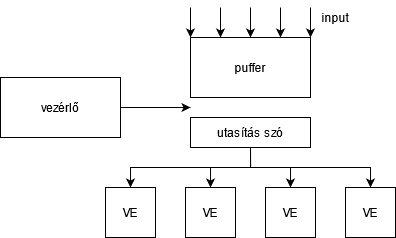
\includegraphics[width=0.6\textwidth]{vliw}
    \centering
    \caption{A VLIW architektúra logikai ábrázolása}
    \label{fig:vliw}
\end{figure}

\section{Első generáció - széles VLIW-ek}
A széles VLIW architektúrákat a 70-es években fejlesztették, nagyjából 10-20 végrehajtó egységgel rendelkeztek.
Az utasítá szavak 256-1024 bit hosszúak volt.
A compilerek ezt még nem tudták kihasználni a kezdetleges függőség kezelés miatt (nem tudták ellátni a CPU-t elegendő független utasítással).

\section{Második generáció - keskeny VLIW-ek}
A 90-es években keskeny VLIW-eket kezdett fejleszteni az Intel és a HP, Itanium Project néven.
Ezek a processzorok 2-8 végrehajtó egységgel rendelkeztek, ami lényegesen nagyobb teljesítményt biztosított a fejlettebb compilerek segítségével, mint a korabeli futószalag processzorok.
A digitális feldolgozás szükségessége szintén segített a keskeny VLIW architektúrák elterjedésében, mivel ilyen feladatoknál nagy mennyiségű független utasítást kell végrehajtani.
Végül a 2000-es évek elején jelentek meg az első ilyen processzorok, 4-8 utasítást tartalmazó utasítás szóval.
Az Intel ezeket EPIC (Explicitly Parallel Instruction Computing) processzoroknak nevezte.
\subsubsection{Jellemzői}
\begin{itemize}
    \item Fordítási időben történő ütemezés $\rightarrow$ nagy mennyiségű tranzisztor szabadul fel.
    \item A plusz tranzisztorokat extra regiszterek kialakítására használták fel.
    \item Regiszterekben gazdag architektúra.
    \item Tervezési elv, hogy a lehető legtöbb utasítás fusson párhuzamosan, akkor is, ha egy részük feleslegesen hajtódik végre.
\end{itemize}
\subsubsection{A tervezési elv előnyei}
\begin{itemize}
    \item Vezérlés függőség (pl. feltételes elágazás) esetén mindkét ág végrehajtásra kerül $\rightarrow$ csökken az elágazási késletetés.
    \item Spekulatív adatbetöltés (optimalizáló compiler funkció - a compiler úgy állítja össze a gépi kódot, hogy amíg pl. egy adat betöltésére várakozik, addig más utasításokat közben végrehajt).
    \item Alkalmas nagy megbízhatóságú szerverekben történő alkalmazásra.
\end{itemize}
\subsubsection{A tervezési elv hátrányai}
\begin{itemize}
    \item Energiapazarló, mobil eszközökben nehezen alkalmazható a nagy fogyasztás miatt. Következmény, hogy elsősorban szerverekben terjedt el.
\end{itemize}

\section{Az IA-64 architektúra}
Az Intel a VLIW architektúra továbbfejlesztéseként megalkotta az "új ISA", azaz az IA-64 architektúrát.
Ez volt az Intel első 64 bites architektúrája, a tervek között szerepelt az x86 kivezetése is, viszont az IA-64 nem volt kompatibilis az x86-ra írt szoftverekkel.
Bár a Windows XP-t még megírták IA-64-re is, a drága gyártásnak és a többmagos, 64 bites, de visszafelé kompatibilis x86\_64-es processzorok megjelenésének köszönhetően a fejlesztést 2016-ban végleg leállították.
Maga a VLIW architektúra egy modern, előre mutató és megbízható rendszer volt, a fejlesztés leállításának okai részben üzletiek voltak (amíg az Intel és a HP az IA-64-et fejlesztette, az AMD megalkotta az x86\_64 architektúrát, ami kompatibilis volt az x86-os szoftverekkel).
Nem kizárható, hogy a jövőben még visszatérnek a VLIW CPU-k.